
\chapter{Introduction}
\label{Chap:Intro}
This thesis considers the problem of tracking human wrist movements during free living.
These movements would need to be tracked cintinuously all day,
storing the data so that it can be processed later.
To capture this information we need an accekerometer and a gyroscope.
Accelerometers typically draw a current of 270$\mu$,
while a gyroscope can consume 3 - 10$\mu$ of current.
These devices are powered by a battery,
and common small batteries used in wrist based devices have a capacity of 20 - 200mAh.
These capacities allow for an accelerometer based device to operate up to a week,
however, depending on the size of the battery,
devices with a gyroscope typically operate for a couple of hours because of their higher current consumption.
The battery size also affects the size of the device as the battery is usually the largest part in the device.
Since we want our device to be mounted on the wrist,
we would like our battery size to be small enough to be comfortably worn on the wrist.

Our group is motivated by the vision of a wrist mounted device that can track wrist motion activity and
detect when a person is eating,
and also be able to count the number of bites in each meal.
In previous research we have demonstrated algorithms where periods of eating can be detected with 81\% accuracy,
and the number of bites in these meals can be detected with 86\% accuracy.
To further this research,
we reqyure a device that will allow us to record wrist motion data for a period of days to weeks and can be used across a large number of subjects.
Due to this extended interval of use,
the device needs a long battery life,
and has to be comfortable to wear.


\section{Motivation}
\label{Sec:Motivation}

 Obesity is an increasing problem. CDC (Centers for Disease Control and Prevention) reports mention one
 \textemdash{} third of the adult American population as 
 obese, while sixty nine percent of the population is considered 
 overweight. The agency defines individuals with a Body Mass
 Index of twenty five and above as overweight~\cite{ogden2010prevalence}.
 This number is rising in children too, with eighteen
 percent children between the ages of 12 \textemdash{} 18
 years considered obese. Modern advances in technology
 have helped our minds act without much thought into our action.
 Consider the example of driving a car, where your thought might drift
 into an event that happened during the day, but you are still able to drive the car.
 Similarly, not only is it easy to order prepared food, but eating
 food while watching television or using a computer makes
 it very easy to consume a large amount of calories quickly without
 noticing it happen. When a group
 of individuals was asked to count the number of bites taken over
 a 24 hour period, 40\% lost count or forgot the count entirely~\cite{mahoney1975obese}.
 The abundance of fast food chains, high calorie food, and soda dispensers makes it very easy
 for a person to consume a large amount of calories without realizing 
 that they are doing so. Children who ate fast food, compared with those who did not,
 consumed an average of 187 kcal more every day~\cite{bowman2004effects}.
 A study has shown that eating slowly is shown to help decrease the amount of calories
 consumed during a meal~\cite{Andrade2008}, however it is not an
 easy change to make in our busy lives, or one that can be sustained.

\begin{figure}
\begin{center}
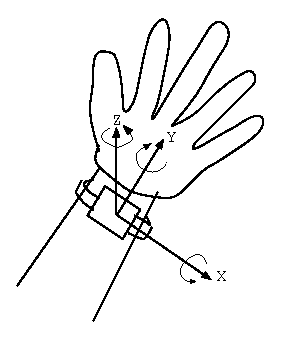
\includegraphics{images/HandAxis.eps}
\caption{A wrist watch shaped device showing the different axis being recorded.}
\label{fig:HandAxis}
\end{center}
\end{figure}
 
 
\section{Fitness Tracking}
\label{Sec:FitnessTracking}
\begin{figure}
%\begin{center}
\centering
\begin{subfigure}[b]{0.4\textwidth}
\includegraphics[width=0.8\textwidth]{images/CCScreenshot.PNG}
\caption{Calorie Counter}
\label{fig:CCScreenshot}
\end{subfigure}
\qquad
\begin{subfigure}[b]{0.4\textwidth}
\includegraphics[width=0.8\textwidth]{images/MyFitScreenshot.png}
\caption{MyFitnessPal}
\label{fig:MyFitScreenshot}
\end{subfigure}
\caption{Screenshots of two famous Fitness Tracking Software}
\label{fig:FitnessScreenshots}
%\end{center}
\end{figure}
With the increase in smart phone sales,
we see a huge rise in small applications that help track our daily activities.
Applications like CalorieCount\footnote{Allows users to name and record calories consumed.
Users can pick from a database or enter their own values.} \cite{Web:CalorieCount} and MyFintessPal
\footnote{Allows users to pick various foods or exercises from a database or enter their own data} \cite{Web:MFP}
allow users to track their daily intake of food and also track other activities like exercise and sleep.
However, this data was still largely dependent on the user's ability to record these events,
and requires frequent user intervention and foresight.
It may be possible to create a device that could detect our movements,
predict what we are doing, and record this information autonomously.
Smaller sensors and components have allowed wearable devices to enter the market,
which allows these devices to be a part of clothing or accessory that contains
a microcomputer. This microcomputer can perform electronic functions that allow it to monitor and
detect human movement. Based on these detections, some kind of action can be performed.
These devices are shown to have a battery life of 24 to 48 hours.

\begin{figure}
\begin{center}
\includegraphics[width=0.4\textwidth]{images/JawFit.png}
\caption{The Fitbit flex (left) activity tracker}
\label{fig:FitbitJawbone}

\end{center}
\end{figure}
Fitness trackers in the market currently offer a range of services. The Fitbit \cite{Web:FitBitOfficial},\cite{Web:FitbitFlex} and Jawbone \cite{Web:JawBoneWebsite} series of sensors allow for exercise and sleep monitoring using wrist movements. This data is then synchronized with a computer or a mobile phone, and can be viewed graphically by the user. Another consumer electronic segment that has now emerged is smart watches. These watches contain electronic components that make them functionally similar to a mobile phone, and are small enough to wear on the wrist. They contain low power displays and have a host of power saving techniques to have a long battery life. However most of the wearable devices in the market are limited to counting the number of calories expended and thus not many options exist for counting the number of calories consumed.

\section{SHIMMER}
\label{Sec:Shimmer}
\begin{figure}
\begin{center}
\includegraphics{images/shimmerphoto.jpg}
\caption{Product photo of the SHIMMER sensing platform.}
\label{Fig:ShimmerHand}
\end{center}
\end{figure}
Our application of using wrist movement to detect bites is very similar to biomedical research where the body is being monitored.
Similar constraints on the size of devices and battery life exist when they have to be used in biomedical research.
Burns et al. have demonstrated a device called the SHIMMER
(an acronym for Sensing Health with Intelligence, Modularity, Mobility and Experiment Resusability)~\cite{burns2010shimmer}.
The device is available in a small form factor (50mm X 25mm X 12.5mm),
and has a battery life of over twenty four hours with data from an accelerometer actively being recorded.
It features an MSP430 Ultra-low power microcontroller,
SD Card for storage,
a Bluetooth module for wireless communication,
and a lightweight battery (15).
It is possible to connect an external sensor to the SHIMMER by using its general purpose I/O pins.
Figure \ref{Fig:ShimmerHand} shows a product photograph of the device from the Shimmer website~\cite{Web:ShimmerBuyKit}.
Power is extended by disabling most components when not needed.
Burns et al. mention that the duty cycle of writing to the memory chip or the Bluetooth module can be reduced to save power,
however this is not possible in situations where the frequency is high because of the wake up time on these modules~\cite{burns2010shimmer}.
Shimmer sensing commercially provides these modules,
and a single base module can be purchased for US \$249~\cite{Web:ShimmerBuy}.
However, to program the SHIMMER base we would need access to the SHIMMER development KIT,
which costs US \$1999, or higher if additional features are required.

\section{Previous Work}
Our group has been involved with bite counting by tracking wrist motion for half a decade.
Initial research~\cite{dong2012new} worked on identifying if this was a feasible idea.
During the early stages,
sensors were mounted directly on the wrist,
and a cable connected the sensor to a personal computer.
The computer would log data from the sensors and identify when the user took a bite of food.
Needless to say,
mobility by the user was limited,
and they would have to consume all of their meal within range of the computer cable.
Later work switched to a device that could process this information from the sensor in real time,
and predict the total number of bites taken by the user in a meal.
This device was able to store only the number of bites, 
but not the actual data captured from the sensors.
It was widely reviewed and reported by the media.
Figure \ref{Fig:BCEater} shows a photograph from the research groups website showing the final device which was mass manufactured.

\begin{figure}
        \centering
        % \begin{subfigure}[b]{0.3\textwidth}
                \includegraphics[]{images/BCEater.JPG}

                \label{fig:gull}
        % \end{subfigure}%
        ~ %add desired spacing between images, e. g. ~, \quad, \qquad, \hfill etc.
          %(or a blank line to force the subfigure onto a new line)
        % \begin{subfigure}[b]{0.3\textwidth}
        %         \includegraphics[width=\textwidth]{images/BCWrist.JPG}
        %         \caption{Close up photo of the bite counter mounted on a wrist.}
        %         \label{fig:tiger}
        % \end{subfigure}
         \caption{Photograph of a person using the Bite Counter while eating.}\label{Fig:BCEater}
\end{figure}

\section{Wearable Wrist Motion Tracker}
\label{Sec:WearbleTracker}
Earlier work by the group showed a device that is capable of detecting bites by monitoring wrist movement~\cite{drennan2010assessment}.
We are motivated by the problem of monitoring calorie consumption by creating a wrist watch like device that automates this process of monitoring wrist movements.
Since the device is to be worn by the user everyday, it needs to be comfortable to wear.
This would required the device to have a small size.
To avoid having to recharge often, or risking the battery dying during a meal,
the device also needs to have a good battery life\footnote{Requiring a recharge not more than once a day}.
Our device records raw inertial movement data (rotation and acceleration), and stores this in a memory chip.
The configuration of the various axes is displayed in Figure \ref{fig:HandAxis}.
The data can later be accessed later using a computer and can processed by algorithms
to detect when a bite of food has been eaten~\cite{dong2012new}.
